\section{Comparaison des performances avec pthread}

Afin d’évaluer notre bibliothèque de threads en espace utilisateur,
    nous l’avons comparée aux pthreads à l’aide du test 61 - mutex,
    qui consiste à incrémenter un compteur partagé protégé par un
        mutex.Chaque thread effectue 1000 incrémentations,
    avec des appels à \texttt{
        thread\_yield()} à l’intérieur de la section critique,
    ce qui force de nombreux changements de contexte et accentue la contention
        sur le verrou.\\

\noindent Avant de présenter les résultats,
    il est important de préciser les conditions expérimentales
        .Les tests ont été réalisés sur une machine disposant
            de 4 cœurs physiques.Or,
    les pthreads peuvent exploiter le parallélisme matériel,
    contrairement à notre implémentation qui repose sur un seul thread
        noyau.Afin de garantir une comparaison équitable,
    nous avons donc limité l’exécution des programmes à un seul cœur à l’aide de
        la commande \texttt{taskset}
            .Ainsi,
    le graphe ci -
        dessous montre les performances en fonction du nombre de threads.

\begin{figure}[h]
	\centering
	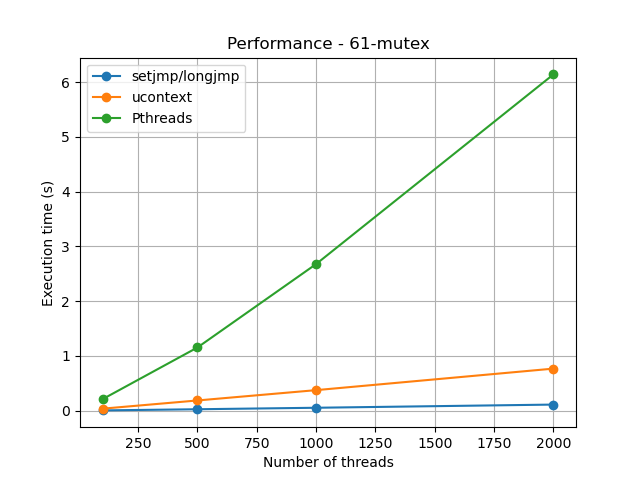
\includegraphics[width=0.9\linewidth]{rapport/images/61-mutex.png}
\caption{Comparaison des performances du test 61-mutex}
\label{fig:61-mutex}
\end{figure}

On observe un écart très important entre les différentes
    implémentations.Par exemple,
    pour 500 threads, notre version basée sur setjmp / longjmp met environ 0,
    0263 s, contre 0, 1868 s pour la version ucontext et 1,
    1547 s pour pthreads.Cet écart augmente avec le nombre de threads
        .\\

\noindent Cette différence s’explique directement par la manière dont le mutex
            et l’ordonnancement sont implémentés.Dans notre bibliothèque,
    les threads sont exécutés en espace utilisateur avec un ordonnancement
        coopératif
    : lorsqu’un thread appelle \texttt{thread\_yield()},
      le changement de contexte est très léger et ne nécessite pas d’appel au
          noyau.De plus,
      le mutex est entièrement géré en espace utilisateur,
      ce qui rend les opérations de verrouillage et déverrouillage très rapides,
      même en cas de forte contention.\\

\noindent À l’inverse,
      les pthreads reposent sur des threads noyau.Chaque contention sur le mutex
          peut entraîner des appels système et des blocages gérés par le noyau,
      ce qui induit un surcoût important.De plus,
      les changements de contexte sont plus lourds car ils impliquent le
          scheduler du système.\

      Enfin,
      la différence entre setjmp /
          longjmp et ucontext provient du fait que ucontext est plus général
              mais aussi plus coûteux,
      ce qui augmente le temps des changements de contexte.
